% Compile from slide/20261107/ (PDF: slide/out/20261107/ , other files: build/):
%   ../lualatex-dated.sh -synctex=1 -interaction=nonstopmode -file-line-error -output-directory=out survey_kawamotostyle_20261107_handout_v5_en.tex
\documentclass[aspectratio=169,10pt,t,handout]{beamer}
\usepackage[en]{labslide}
% Raise every requested font size by 1pt, as in the Japanese handout.
\makeatletter
\newdimen\labvtwo@size
\newskip\labvtwo@skip
\let\labvtwo@set@fontsize\set@fontsize
\def\set@fontsize#1#2#3{%
  \@defaultunits\labvtwo@size#2pt\relax\@nnil
  \advance\labvtwo@size by 1pt\relax
  \@defaultunits\labvtwo@skip#3pt\relax\@nnil
  \advance\labvtwo@skip by 1pt\relax
  \begingroup
    \edef\x{\endgroup
      \noexpand\labvtwo@set@fontsize{\unexpanded{#1}}{\strip@pt\labvtwo@size}{\the\labvtwo@skip}%
    }\x
}
\makeatother
\usetikzlibrary{fit,backgrounds,calc,positioning}

\makeatletter
\setlength{\beamer@frametopskip}{0mm}
\makeatother
\setbeamertemplate{frametitle}{%
  \vspace{4.2mm}%
  {\usebeamerfont{frametitle}\color{ink}\insertframetitle\par}%
  \vspace{0.4mm}%
  {\color{ruleblue}\rule{\textwidth}{0.7pt}\par}%
  \vspace{1.1mm}%
  \ifx\insertframesubtitle\@empty\else
    {\footnotesize\color{muted}\insertframesubtitle\par}%
    \vspace{1.2mm}%
  \fi
}

\definecolor{cviolet}{HTML}{F3E8F6}
\definecolor{cviolettt}{HTML}{7A458E}
\definecolor{cred}{HTML}{F8E6E6}
\definecolor{credtt}{HTML}{C44545}
\renewcommand{\usecardcolor}[1]{%
  \def\cardfill{cgreen}%
  \def\cardtitlec{cgreentt}%
  \ifstrequal{#1}{red}{%
    \def\cardfill{cred}%
    \def\cardtitlec{credtt}%
  }{}%
  \ifstrequal{#1}{orange}{%
    \def\cardfill{corange}%
    \def\cardtitlec{corangett}%
  }{}%
  \ifstrequal{#1}{blue}{%
    \def\cardfill{cblue}%
    \def\cardtitlec{cbluett}%
  }{}%
  \ifstrequal{#1}{green}{%
    \def\cardfill{cgreen}%
    \def\cardtitlec{cgreentt}%
  }{}%
  \ifstrequal{#1}{violet}{%
    \def\cardfill{cviolet}%
    \def\cardtitlec{cviolettt}%
  }{}%
  \ifstrequal{#1}{plain}{%
    \def\cardfill{cplain}%
    \def\cardtitlec{cplaintt}%
  }{}%
  \ifstrequal{#1}{gray}{%
    \def\cardfill{cplain}%
    \def\cardtitlec{cplaintt}%
  }{}%
}

\graphicspath{{fig/}{../20261007/fig/survey/}}

\kicker{Survey}
\title{A local planner for both\\safety and preference}
\subtitle{CATNAV and SEA-Nav}
\date{November 2026}

\newcommand{\li}{%
  \ifvmode\else\par\fi
  \noindent\hangindent=1.15em\hangafter=1
  \makebox[1.15em][l]{\textcolor{ruleblue}{\textbullet}}\ignorespaces}
\newcommand{\lii}{%
  \ifvmode\else\par\fi
  \noindent\hspace{1.0em}\hangindent=2.15em\hangafter=1
  \makebox[1.05em][l]{\textcolor{muted}{\textendash}}\ignorespaces}
% An equation under a bullet, indented, and not itself a bullet.
\newcommand{\lieq}[1]{%
  \par\nobreak
  \noindent\hangindent=2.3em\hangafter=1
  \hspace*{2.3em}{\scriptsize #1}\ignorespaces}

\newcommand{\cardbalance}{\par\vspace*{-\topskip}\vspace{0pt plus 1fill}}
\newcommand{\takeawaybalance}[1]{%
  \par\vspace{0.15em plus 1fill}%
  \begingroup
  \setlength{\fboxsep}{5pt}%
  \noindent\colorbox{ink}{%
    \parbox[c]{\dimexpr\textwidth-10pt\relax}{%
      \color{white}\footnotesize #1}}%
  \endgroup
}

\RenewDocumentCommand{\infocard}{O{green} o m m}{%
  \usecardcolor{#1}%
  \IfValueTF{#2}{\def\cardminh{#2}}{\def\cardminh{0pt}}%
  \begin{tikzpicture}[baseline=(card.north)]
    \node[
      anchor=north west,
      fill=\cardfill,
      text width=\dimexpr\linewidth-14pt\relax,
      minimum height=\cardminh,
      inner xsep=6.5pt,
      inner ysep=4pt,
      align=flush left
    ] (card) {%
      {\color{\cardtitlec}\bfseries #3}\par\vspace{0.15em}%
      {\color{body}\footnotesize #4\par}%
    };
  \end{tikzpicture}%
}

% Zero-shot perception. #1 = none colors every node the same; otherwise only that node is orange.
\newcommand{\flowhl}{none}
\newcommand{\flownode}[3]{%
  \ifdefstring{\flowhl}{#1}{%
    \node[kworange, line width=1.05pt, flown] (#1) at #2 {#3};%
  }{%
    \ifdefstring{\flowhl}{none}{%
      \node[kwblue, flown] (#1) at #2 {#3};%
    }{%
      \node[kwblue, opacity=0.38, text opacity=1, flown] (#1) at #2 {#3};%
    }%
  }%
}
\newcommand{\cacheflow}[1][none]{%
  \renewcommand{\flowhl}{#1}%
  \begin{tikzpicture}[
      flown/.style={align=center, text width=24mm, minimum height=12mm, inner sep=1.6pt, font=\scriptsize},
      lbl/.style={font=\scriptsize, text=muted, align=center, inner sep=1pt}
    ]
    \flownode{clip}{(0,4.55)}{CLIP Encoder\\Image feature}
    \flownode{vlm}{(2.55,4.55)}{VLM\\Object risk}
    \flownode{cache}{(1.28,2.25)}{Cache}
    \flownode{seg}{(0,0)}{CLIP-Seg\\Segmentation}
    \flownode{map}{(2.55,0)}{Cost map}
    \coordinate (cinL) at ($(cache.north west)!0.42!(cache.north east)$);
    \coordinate (cinR) at ($(cache.north west)!0.58!(cache.north east)$);
    \coordinate (coutL) at ($(cache.south west)!0.42!(cache.south east)$);
    \coordinate (coutR) at ($(cache.south west)!0.58!(cache.south east)$);
    \draw[kwarr] (clip.south) -- (cinL)
      node[lbl, midway, left] {feature};
    \draw[kwarr] (vlm.south) -- (cinR)
      node[lbl, midway, right] {cost table};
    \draw[kwarr] (coutL) -- (seg.north)
      node[lbl, midway, left] {names};
    \draw[kwarr] (coutR) -- (map.north)
      node[lbl, midway, right] {risk};
  \end{tikzpicture}%
}

% Standard actor-critic and SEA-Nav. The value arrow leaves the critic.
\newcommand{\acdiagram}{%
  \begin{tikzpicture}[
      font=\scriptsize,
      box/.style={align=center, minimum height=9.5mm, text width=23mm, inner sep=1.8pt},
      env/.style={box, text width=20mm, kw, draw=cplaintt, fill=cplain},
      act/.style={box, kwblue},
      cri/.style={box, kwgreen},
      lse/.style={box, text width=24mm, kworange}
    ]
    \node[font=\scriptsize\bfseries, text=muted] (t1) at (1.7,2.35) {Standard actor-critic};
    \node[env] (e1) at (0,0.9) {Environment};
    \node[act] (a1) at (3.35,0.9) {Actor: action};
    \node[cri] (c1) at (3.35,-1.05) {Critic: value};
    \draw[kwarr] (e1.east) -- (a1.west);
    \draw[kwarr] (e1.south) -- (e1.south |- c1.west) -- (c1.west);
    \draw[kwarr] (c1.north) -- (a1.south)
      node[midway, right, font=\scriptsize, text=ink] {value};

    \node[font=\scriptsize\bfseries, text=cbluett] at (8.35,2.35) {SEA-Nav};
    \node[env] (e2) at (6.45,0.9) {Environment};
    \node[act] (a2) at (9.50,0.9) {Actor: action};
    \node[lse] (s) at (12.58,0.9) {LSE-CBF\\Safe action};
    \node[cri] (c2) at (9.50,-1.05) {Critic: value};
    \draw[kwarr] (e2.east) -- (a2.west);
    \draw[kwarr] (e2.south) -- (e2.south |- c2.west) -- (c2.west);
    \draw[kwarr] (a2.east) -- (s.west);
    \draw[kwarr] (c2.east) -- node[below, font=\scriptsize, text=ink] {value} (c2.east -| s.south) -- (s.south);
  \end{tikzpicture}%
}

\begin{document}

\begin{frame}[plain]
  \labtitlepage{}
\end{frame}

\begin{frame}{Research theme | Robot control}
  \centering
  \begin{tikzpicture}[node distance=5.5mm]
    \node[kworange, text width=28mm, minimum height=8mm] (c) {Controller};
    \node[kwgreen, text width=28mm, minimum height=8mm, right=of c] (p) {Local planner};
    \node[kwblue, text width=26mm, minimum height=8mm, right=of p] (g) {Gait model};
    \node[kwpurple, text width=22mm, minimum height=8mm, right=of g] (m) {Motor};
    \draw[kwarr] (c) -- (p)
      node[midway, below=4mm, font=\scriptsize, text=muted] {target pose};
    \draw[kwarr] (p) -- (g)
      node[midway, below=4mm, font=\scriptsize, text=muted] {target speed};
    \draw[kwarr] (g) -- (m)
      node[midway, below=4mm, font=\scriptsize, text=muted] {torque};
  \end{tikzpicture}

  \vspace{1.5em}
  \includegraphics[width=\textwidth,height=35mm,keepaspectratio]{img001.png}

  \takeaway{In general, the input reaches the motors through three transforms.}
\end{frame}

\begin{frame}{Research theme | Local planner}
  \centering
  \begin{tikzpicture}[node distance=5.5mm]
    \node[kworange, text width=28mm, minimum height=8mm, opacity=0.2] (c) {Controller};
    \node[kwgreen, text width=28mm, minimum height=8mm, right=of c] (p) {Local planner};
    \node[kwblue, text width=26mm, minimum height=8mm, right=of p] (g) {Gait model};
    \node[kwpurple, text width=22mm, minimum height=8mm, right=of g, opacity=0.2] (m) {Motor};
    \draw[kwarr] (c) -- (p)
      node[midway, below=4mm, font=\scriptsize, text=muted] {target pose};
    \draw[kwarr] (p) -- (g)
      node[midway, below=4mm, font=\scriptsize, text=muted] {target speed};
    \draw[kwarr] (g) -- (m)
      node[midway, below=4mm, font=\scriptsize, text=muted] {torque};
  \end{tikzpicture}

  \includegraphics[width=\textwidth,height=35mm,keepaspectratio]{img002.png}

  \takeaway{Study a local planner that sets the target speed for both safety and preference.}
\end{frame}

\begin{frame}{Papers on preference and safety}
  \infocard[green][24mm]{Preference | CATNAV}{%
    \li Cached Vision-Language Traversability for Efficient Zero-Shot Robot Navigation
    \li Potnis et al., arXiv, 2026
    \li A VLM estimates semantic risk and picks a preferred path from several candidates.}
  \vspace{0.4em}
  \infocard[blue][24mm]{Safety | SEA-Nav}{%
    \li Efficient Policy Learning for Safe and Agile Quadruped Navigation in Cluttered Environments
    \li Chen et al., arXiv, 2026
    \li A differentiable safety filter sits inside the policy and learns cluttered scenes quickly.}

  \takeaway{The first paper puts preference in the path choice. The second puts safety in the velocity command.}
\end{frame}

% ---------- CATNAV ----------

\begin{frame}{CATNAV}
  \source{Potnis et al., arXiv, 2026, Fig.~1}
  \vspace*{0.2em plus 1fill}
  \begin{columns}[T,onlytextwidth]
    \begin{column}{0.32\textwidth}
      \centering
      \begin{minipage}[t][40mm][c]{\linewidth}
        \centering
        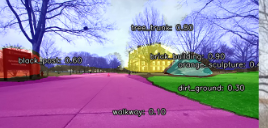
\includegraphics[width=\linewidth,height=38mm,keepaspectratio]{catnav_clipseg.png}
      \end{minipage}\\[0.25em]
      {\scriptsize CLIP Seg}
    \end{column}
    \hfill
    \begin{column}{0.32\textwidth}
      \centering
      \begin{minipage}[t][40mm][c]{\linewidth}
        \centering
        
\includegraphics[width=\linewidth,height=38mm,keepaspectratio]{catnav_costmap_inset.png}
      \end{minipage}\\[0.25em]
      {\scriptsize Cost map}
    \end{column}
    \hfill
    \begin{column}{0.32\textwidth}
      \centering
      \begin{minipage}[t][40mm][c]{\linewidth}
        \centering
        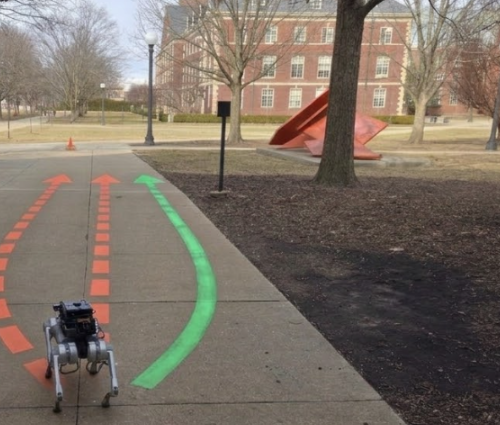
\includegraphics[width=\linewidth,height=38mm,keepaspectratio]{catnav_select.png}
      \end{minipage}\\[0.25em]
      {\scriptsize Select Route}
    \end{column}
  \end{columns}
  \vspace*{0.15em plus 1fill}

  \takeaway{Preference is chosen in two stages: segment the scene, build a cost map, then pick one path.}
\end{frame}

\begin{frame}{Background}
  \source{Potnis et al., arXiv, 2026}
  \infocard[gray][20mm]{Traversability risk}{%
    \li Judge it against what the robot can physically do
    \li Outdoors, account for moving obstacles and terrain
    \li Indoors, account for people and fragile objects}
  \vspace{0.7em}
  \begin{columns}[T,onlytextwidth]
    \begin{column}{0.305\textwidth}
      \infocard[orange][24mm]{Learning-based}{%
        \li Needs a large training set
        \li Weak out of distribution}
    \end{column}
    \hfill
    \begin{column}{0.305\textwidth}
      \infocard[blue][24mm]{VLM}{%
        \li A cost can lose flexible reasoning
        \li A call every frame is expensive}
    \end{column}
    \hfill
    \begin{column}{0.305\textwidth}
      \infocard[green][24mm]{VLA}{%
        \li Can output velocity directly
        \li Hard to see why that path was chosen}
    \end{column}
  \end{columns}

  \takeaway{Keep both a number and a human-like judgment, with little data and little compute.}
\end{frame}

\begin{frame}{Challenges}
  \source{Potnis et al., arXiv, 2026}
  \cardbalance
  \infocard[blue][16mm]{Challenge 1}{%
    \li Strong reasoning, even with few annotations}
  \vspace{0.28em}
  \infocard[orange][16mm]{Challenge 2}{%
    \li A high rate, even with limited compute}
  \vspace{0.28em}
  \infocard[green][16mm]{Challenge 3}{%
    \li Social and flexible judgment, not only numbers}
  \takeawaybalance{Preferably, a person can interpret that judgment.}
\end{frame}

\begin{frame}{Contributions}
  \source{Potnis et al., arXiv, 2026}
  \cardbalance
  \infocard[blue][16mm]{Contribution 1 | Zero-shot risk}{%
    \li No task-specific training. A VLM infers a semantic risk.}
  \vspace{0.28em}
  \infocard[orange][16mm]{Contribution 2 | Reused evaluations}{%
    \li Match similar scenes by image features, cache the risk, and query less.}
  \vspace{0.28em}
  \infocard[green][16mm]{Contribution 3 | Path selection}{%
    \li Show several paths on the RGB image and let the VLM pick a visually safe one.}
  \takeawaybalance{Keep the VLM's flexible reasoning without labels, and cut the queries it must answer.}
\end{frame}

\begin{frame}{Method}
  \source{Potnis et al., arXiv, 2026, Fig.~2}
  \centering
  \begin{tikzpicture}
    \node[inner sep=0] (f) {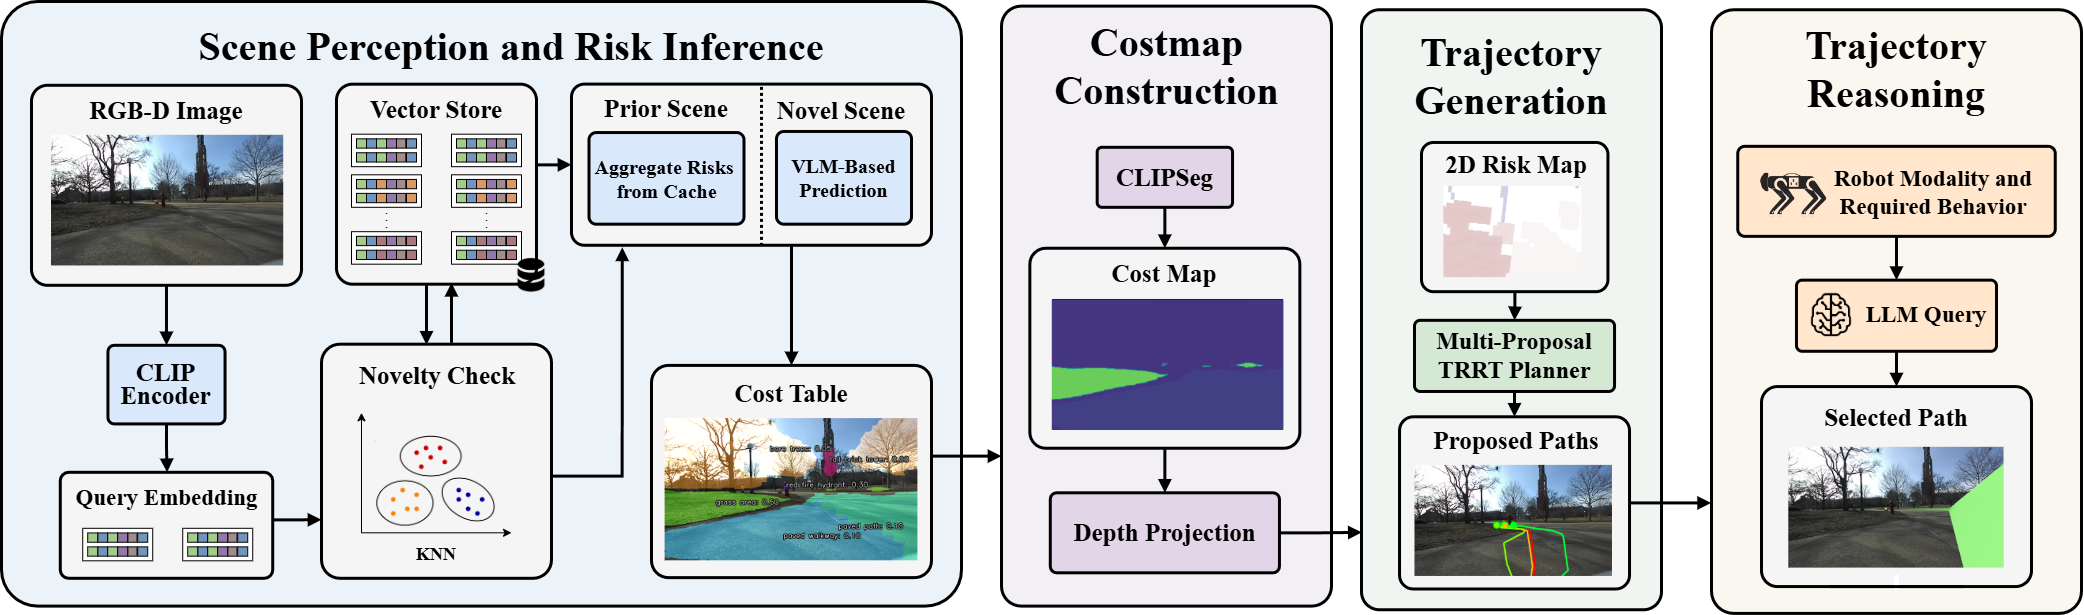
\includegraphics[width=\textwidth,height=40mm,keepaspectratio]{catnav_pipeline.png}};
    \node[anchor=north, font=\scriptsize\bfseries, text=cbluett, align=center]
      at ($(f.south west)!0.22!(f.south east)+(0,-1.6mm)$) {Zero-shot\\perception};
    \node[anchor=north, font=\scriptsize\bfseries, text=corangett, align=center]
      at ($(f.south west)!0.62!(f.south east)+(0,-1.6mm)$) {Risk-based\\path generation};
    \node[anchor=north, font=\scriptsize\bfseries, text=cgreentt, align=center]
      at ($(f.south west)!0.86!(f.south east)+(0,-1.6mm)$) {Flexible\\path selection};
  \end{tikzpicture}

  \takeaway{The action is decided in order: perceive, generate paths, then select one.}
\end{frame}

\begin{frame}{Zero-shot perception}
  \source{Potnis et al., arXiv, 2026}
  \centering
  \scalebox{0.94}{\cacheflow}

  \takeaway{Features and the cost table meet in the cache, and the map is built from there.}
\end{frame}

\begin{frame}{Contribution 1 | Risk from the VLM}
  \source{Potnis et al., arXiv, 2026}
  \begin{columns}[T,onlytextwidth]
    \begin{column}{0.56\textwidth}
      \infocard[blue][28mm]{Cost table}{%
        \li Ask for the object names in the image and their risks
        \li Use no task-specific training data
        \li The call is expensive}
      \vspace{0.35em}
      {\footnotesize\color{body}
      The cost table pairs each object name $c_k$ with a risk $r_k\in[0,1]$.
      \[
        T=\{(c_k,r_k)\}_{k=1}^{K}
      \]}
    \end{column}
    \hfill
    \begin{column}{0.40\textwidth}
      \centering
      \scalebox{0.78}{\cacheflow[vlm]}
    \end{column}
  \end{columns}

  \takeaway{The VLM can estimate risk from its own knowledge, but not on every frame.}
\end{frame}

\begin{frame}{Contribution 2 | CLIP encoder | Image features}
  \source{Potnis et al., arXiv, 2026}
  \begin{columns}[T,onlytextwidth]
    \begin{column}{0.56\textwidth}
      \infocard[blue][22mm]{Features}{%
        \li CLIP encodes the image as a 768-D vector $z_q$
        \li Compare its distance with cached features $z_i$}
      \vspace{0.2em}
      {\footnotesize\color{body}
      $\gamma$ is the novelty threshold. A scene is new only when $d_{\min}$ exceeds $\gamma$.
      \[
        d_{\min}=\min_i\|z_q-z_i\|_2
      \]
      \[
        d_{\min}\le\gamma \;\Rightarrow\; \text{mean risk of $k$ neighbors}
      \]
      \[
        d_{\min}>\gamma \;\Rightarrow\; \text{ask the VLM for the risk}
      \]}
    \end{column}
    \hfill
    \begin{column}{0.40\textwidth}
      \centering
      \scalebox{0.78}{\cacheflow[clip]}
    \end{column}
  \end{columns}

  \takeaway{A close image feature reuses a past risk, which cuts both compute and delay.}
\end{frame}

\begin{frame}{CLIP-Seg | Segmentation}
  \source{Potnis et al., arXiv, 2026}
  \begin{columns}[T,onlytextwidth]
    \begin{column}{0.56\textwidth}
      \infocard[blue][24mm]{Text and pixels}{%
        \li A per-pixel response $p_k(u,v)$ to each object name
        \li The strongest response becomes that pixel's class
        \li Bilinear interpolation lifts the low-resolution response to image size}
      \vspace{0.3em}
      {\footnotesize\color{body} Zero-shot class assignment
      \[
        k^{\star}(u,v)=\arg\max_k p_k(u,v)
      \]}
    \end{column}
    \hfill
    \begin{column}{0.40\textwidth}
      \centering
      \scalebox{0.78}{\cacheflow[seg]}
    \end{column}
  \end{columns}

  \takeaway{Segment with no task labels, by the strongest response to an object name.}
\end{frame}

\begin{frame}{CLIP-Seg | Cost map}
  \source{Potnis et al., arXiv, 2026}
  \begin{columns}[T,onlytextwidth]
    \begin{column}{0.56\textwidth}
      \infocard[blue][20mm]{Pixels and cost}{%
        \li Paint each class risk onto the pixels to build a cost map
        \li Use depth to drop the 3D scene onto a 2D cost map}
      \vspace{0.25em}
      {\footnotesize\color{body}
      Paint the risk only where confidence exceeds $\delta$.
      \[
        M(u,v)=
        \begin{cases}
          r_{k^{\star}} & \text{if } p_{k^{\star}}(u,v)>\delta \\
          0 & \text{otherwise}
        \end{cases}
      \]
      Example: pavement $0.1$, grass $0.3$, people and structures $0.7$.}
    \end{column}
    \hfill
    \begin{column}{0.40\textwidth}
      \centering
      \scalebox{0.78}{\cacheflow[map]}
    \end{column}
  \end{columns}

  \takeaway{Put a cost on each region, project it from 3D to 2D, and use that map.}
\end{frame}

\begin{frame}{Contribution 3 | Generating and selecting paths}
  \source{Potnis et al., arXiv, 2026, Fig.~2}
  \begin{columns}[T,onlytextwidth]
    \begin{column}{0.54\textwidth}
      \infocard[orange][10mm]{1. Center}{%
        \li Build the path with transition-based RRT (T-RRT)}
      \vspace{0.18em}
      \infocard[blue][10mm]{2. Left}{%
        \li Shift the center left by at most $d$, within the safety limits}
      \vspace{0.18em}
      \infocard[green][10mm]{3. Right}{%
        \li Shift the center right by at most $d$, within the safety limits}
      \vspace{0.18em}
      \infocard[violet][10mm]{4. Risky path}{%
        \li Rerun T-RRT with a looser safety threshold}
    \end{column}
    \hfill
    \begin{column}{0.42\textwidth}
      \centering
      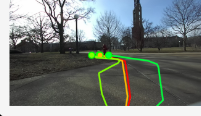
\includegraphics[width=\linewidth]{catnav_paths.png}\\[0.25em]
      {\scriptsize Red: center. Green: sides. Yellow: risky path.}
    \end{column}
  \end{columns}

  \takeaway{Build several paths, then ask the VLM which kind of path is safe, and why.}
\end{frame}

\begin{frame}{Result 1 | Cost from the VLM}
  \source{Potnis et al., arXiv, 2026, Fig.~5}
  \centering
  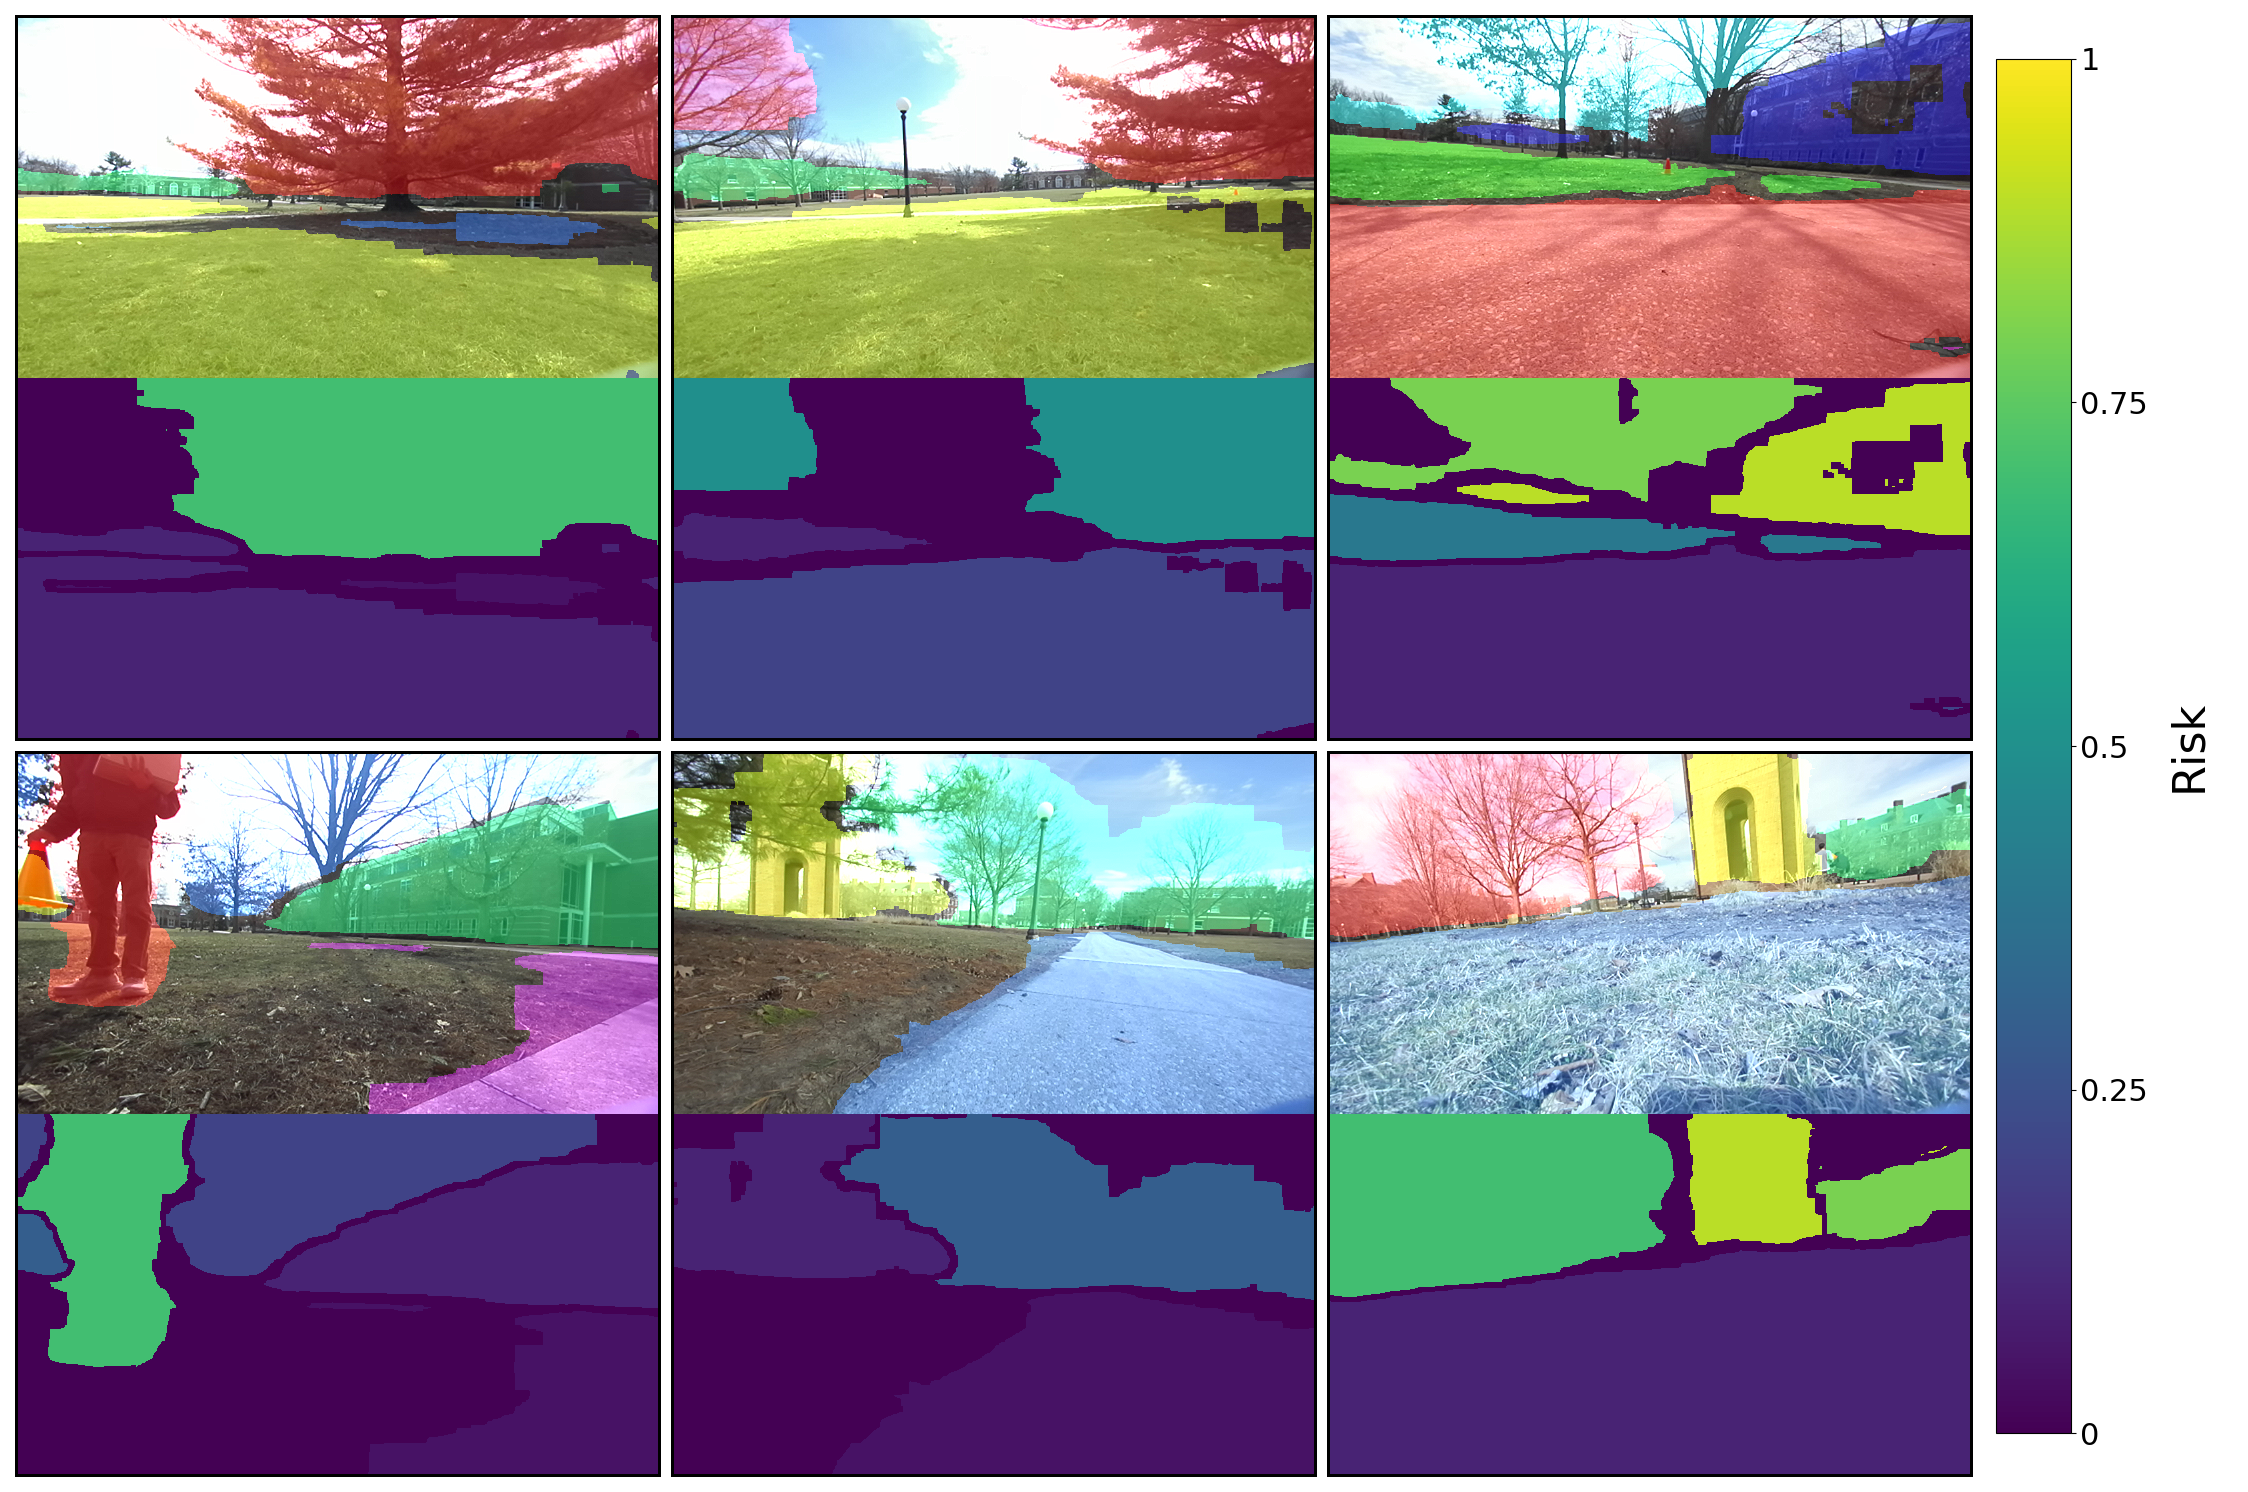
\includegraphics[height=46mm]{catnav_cost.png}

  \vspace{0.15em}
  {\footnotesize Top: segmentation. Bottom: cost.}

  \takeaway{Each region receives a cost. People and structures get a fairly high risk.}
\end{frame}

\begin{frame}{Result 2 | Fewer queries to the VLM}
  \source{Potnis et al., arXiv, 2026, Table~II}
  \begin{columns}[T,onlytextwidth]
    \begin{column}{0.58\textwidth}
      \centering
      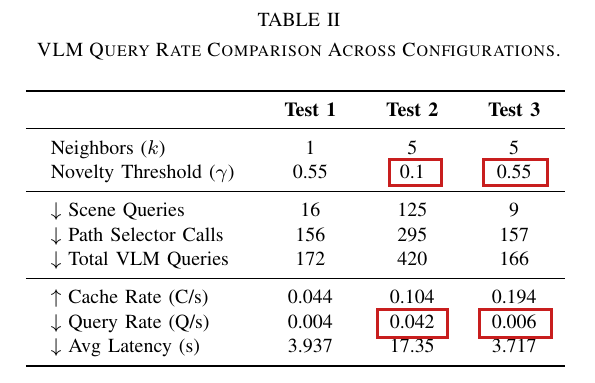
\includegraphics[height=38mm]{catnav_table2.png}
    \end{column}
    \hfill
    \begin{column}{0.40\textwidth}
      \infocard[plain]{Setup}{%
        \li $k$ is how many neighbors are read from the cache
        \li $\gamma$ is the novelty threshold. Query the VLM only if $d_{\min}>\gamma$.}
      \vspace{0.28em}
      \infocard[orange]{Test 2 and Test 3}{%
        \li Test 2 uses a small $\gamma$, so many images count as new
        \li Test 3 restores the threshold at the same $k=5$ and cuts queries by 85.7\%}
    \end{column}
  \end{columns}

  \takeaway{Tuning the novelty threshold reduces how often the image is sent to the VLM.}
\end{frame}

\begin{frame}{Results | Flexible path selection}
  \source{Potnis et al., arXiv, 2026, Table~III, Fig.~6}
  \begin{columns}[c,onlytextwidth]
    \begin{column}{0.54\textwidth}
      \centering
      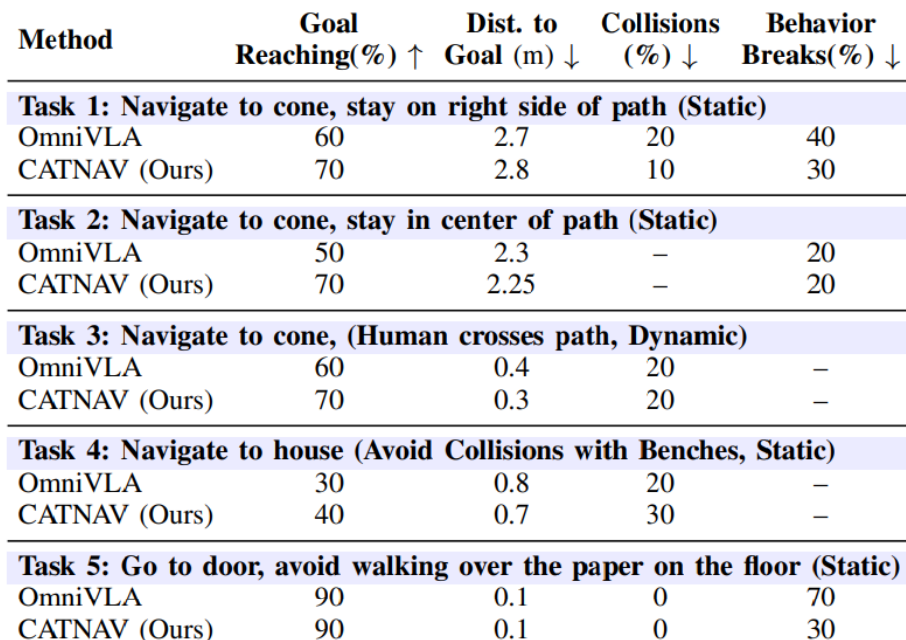
\includegraphics[height=50mm]{survey_table3.png}
    \end{column}
    \hfill
    \begin{column}{0.44\textwidth}
      \centering
      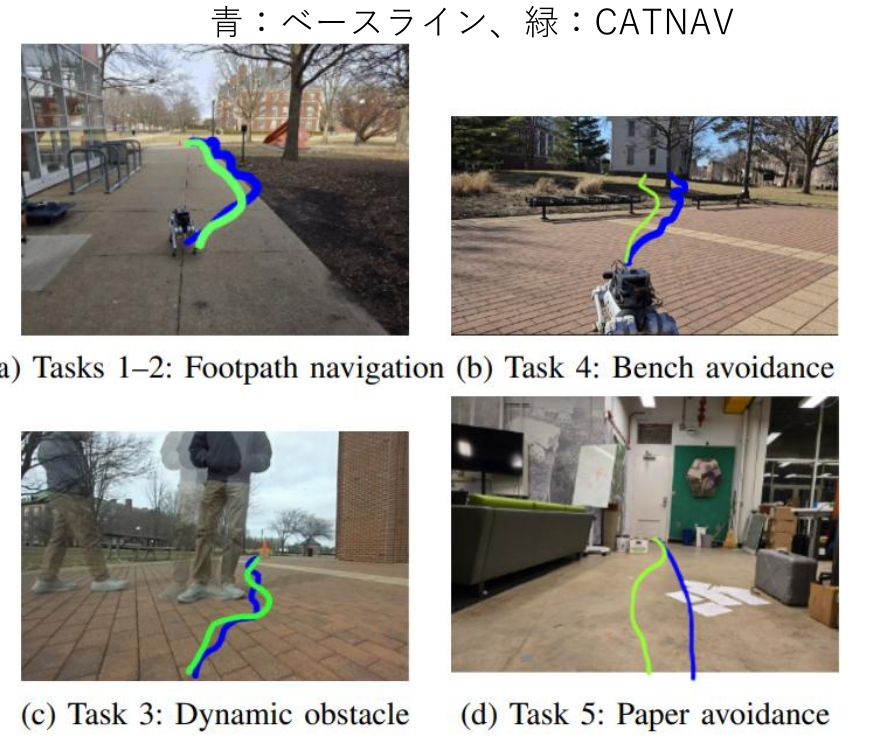
\includegraphics[height=50mm]{survey_trajs.png}
    \end{column}
  \end{columns}

  \takeaway{Success rises by about 10\%. Violations drop, and the robot acts more like a person, such as avoiding paper.}
\end{frame}

\begin{frame}{Summary | CATNAV}
  \source{Potnis et al., arXiv, 2026}
  \begin{columns}[T,onlytextwidth]
    \begin{column}{0.56\textwidth}
      \infocard[blue][14mm]{Contribution 1 | Zero-shot risk}{%
        \li No task training. Each region gets a cost, and people and structures are high.}
      \vspace{0.2em}
      \infocard[orange][14mm]{Contribution 2 | Reused evaluations}{%
        \li Similar scenes are cached. Test 3 cuts VLM queries by 85.7\% relative to Test 2.}
      \vspace{0.2em}
      \infocard[green][14mm]{Contribution 3 | Path selection}{%
        \li Pick one path and give a reason. Success is 68\% versus 58\%, and violations are 33\% lower.}
    \end{column}
    \hfill
    \begin{column}{0.42\textwidth}
      \infocard[orange][48mm]{Limitations}{%
        \li The 2D--3D projection is noisy
        \li A few path parameters are fixed
        \li It needs a capable foundation model, such as CLIP-Seg}
    \end{column}
  \end{columns}

  \takeaway{Preference appears twice: as a numeric cost, then as a visual choice among paths.}
\end{frame}

% ---------- SEA-Nav ----------

\begin{frame}{SEA-Nav}
  \source{Chen et al., arXiv, 2026}
  \centering
  \scalebox{0.95}{\acdiagram}

  \vspace{0.35em}
  {\footnotesize\color{body}
  A standard critic scores the actor's action. SEA-Nav scores the action after LSE-CBF.}

  \takeaway{The safety filter is part of the policy, so the error flows through it.}
\end{frame}

\begin{frame}{Background}
  \source{Chen et al., arXiv, 2026}
  \infocard[orange][18mm]{Autonomous navigation}{%
    \li Dense obstacles make travel hard, so safety has to improve
    \li Large-scale pretraining has raised performance in local scenes}
  \vspace{0.3em}
  \infocard[blue][20mm]{Safe navigation and CBFs}{%
    \li A CBF outside the actor-critic leaves the policy unaware of the correction
    \li If failure ends the episode, the moments just before it are hard to learn from
    \li Few failure samples can be collected}

  \takeaway{Learn the filter's interventions too, and sample efficiently around collisions.}
\end{frame}

\begin{frame}{Prior methods}
  \source{Chen et al., arXiv, 2026}
  \infocard[gray][18mm]{Safety in learned navigation}{%
    \li The robot must pass dense obstacles without a collision
    \li The policy itself must be able to learn the safety intervention}
  \vspace{0.35em}
  \begin{columns}[T,onlytextwidth]
    \begin{column}{0.305\textwidth}
      \infocard[orange][22mm]{Imitation}{%
        \li Copies demonstrated actions
        \li Fails when the scene is new}
    \end{column}
    \hfill
    \begin{column}{0.305\textwidth}
      \infocard[blue][22mm]{Deep RL}{%
        \li Agile in open space
        \li Fails in dense clutter
        \li A safety limit is hard}
    \end{column}
    \hfill
    \begin{column}{0.305\textwidth}
      \infocard[green][22mm]{Post-process}{%
        \li CBF sits outside the actor
        \li The policy does not see it
        \li The correction is not learned}
    \end{column}
  \end{columns}

  \takeaway{Sample efficiency and safe control that includes the filter are both required.}
\end{frame}

\begin{frame}{Contributions}
  \source{Chen et al., arXiv, 2026}
  \cardbalance
  \infocard[blue][16mm]{Contribution 1 | End-to-end LSE-CBF}{%
    \li Smooth the safety condition and remove the mismatch between training and test.}
  \vspace{0.28em}
  \infocard[orange][16mm]{Contribution 2 | Kinematic regularization}{%
    \li Put speed limits and smooth changes in the loss, so the policy transfers safely.}
  \vspace{0.28em}
  \infocard[green][16mm]{Contribution 3 | ACSI}{%
    \li Roll back through the collision and learn, easing the sample bottleneck.}
  \takeawaybalance{A safety layer, regularization, and reused collisions let it traverse after a short run.}
\end{frame}

\begin{frame}{Model structure}
  \source{Chen et al., arXiv, 2026, Fig.~2}
  \centering
  \begin{tikzpicture}
    \node[inner sep=0] (fig) {%
      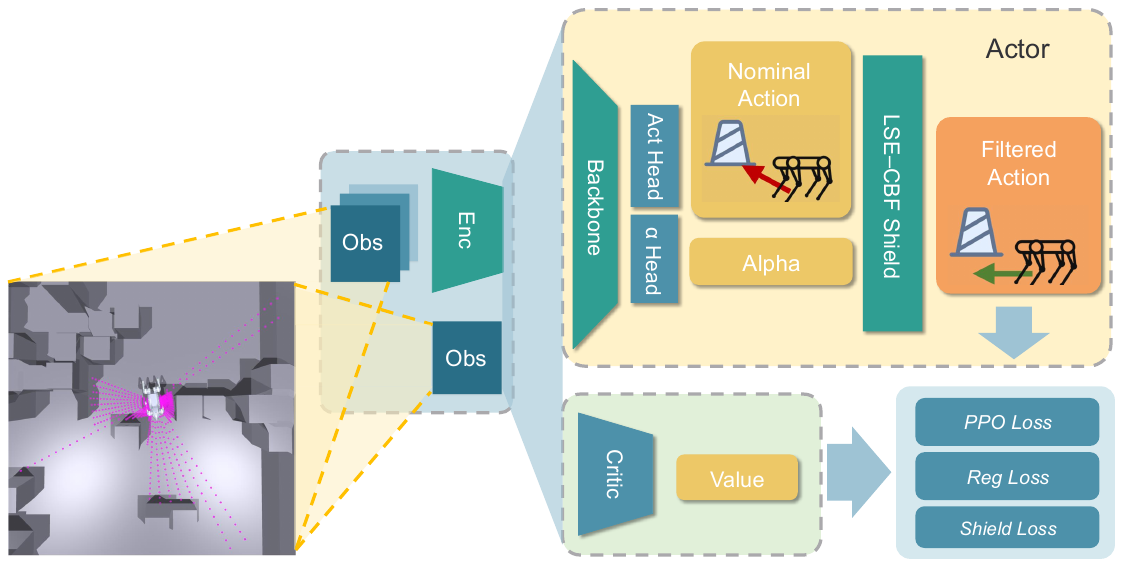
\includegraphics[height=44mm]{seanav_arch.png}};
    \coordinate (featT) at ($(fig.north west)!0.39!(fig.north east)$);
    \coordinate (featB) at ($(fig.south west)!0.39!(fig.south east)$);
    \node[anchor=south, inner sep=0.4pt, font=\scriptsize\bfseries, text=ink]
      at ($(featT)!0.268!(featB)$) {Features};
    \node[anchor=south, font=\scriptsize\bfseries, text=ink]
      at ($(fig.north west)!0.74!(fig.north east)+(0,0.5mm)$) {Actor with CBF};
    \node[anchor=north, inner sep=1pt, font=\scriptsize\bfseries, text=cgreentt]
      at ($(fig.south west)!0.55!(fig.south east)+(0,-0.3mm)$) {Critic};
  \end{tikzpicture}

  \takeaway{The actor outputs a desired speed and $\alpha$, and the loss trains the speed after LSE-CBF.}
\end{frame}

\begin{frame}{How this differs from a standard actor-critic}
  \source{Chen et al., arXiv, 2026}
  \centering
  \scalebox{0.82}{\acdiagram}

  \vspace{0.15em}
  \begin{tikzpicture}[x=8mm, y=7mm, font=\scriptsize]
    \node[text=corangett] at (1.3,1.45) {Heads for the obstacle};
    \draw[-{Stealth[length=1.6mm]}, draw=corangett, line width=0.75pt] (0.15,0.4) -- (1.85,0.4);
    \draw[fill=corange, draw=corangett] (2.25,0.02) -- (2.7,0.95) -- (3.15,0.02) -- cycle;
    \node[text=muted] at (2.7,-0.28) {Obstacle};

    \begin{scope}[xshift=58mm]
      \node[text=cgreentt] at (1.5,1.45) {Can avoid it};
      \draw[-{Stealth[length=1.6mm]}, draw=cgreentt, line width=0.75pt]
        (0.15,0.28) .. controls (1.15,0.28) and (1.2,1.2) .. (2.25,1.05);
      \draw[fill=corange, draw=corangett] (1.85,0.02) -- (2.3,0.95) -- (2.75,0.02) -- cycle;
      \node[text=muted] at (2.3,-0.28) {Obstacle};
    \end{scope}
  \end{tikzpicture}

  \takeaway{SEA-Nav moves an action that heads into an obstacle into the safe set, then scores that action.}
\end{frame}

\begin{frame}{What the actor decides}
  \source{Chen et al., arXiv, 2026, Fig.~2}
  \begin{columns}[T,onlytextwidth]
    \begin{column}{0.50\textwidth}
      \infocard[blue][22mm]{Input}{%
        \li Features from 10 frames of action history
        \li The current observation
        \lii Distance to obstacles along 41 rays}
      \vspace{0.25em}
      \infocard[green][18mm]{Output}{%
        \li Desired velocity command $\bar{u}$
        \li Parameter $\alpha$ of the CBF safety constraint}
    \end{column}
    \hfill
    \begin{column}{0.46\textwidth}
      \centering
      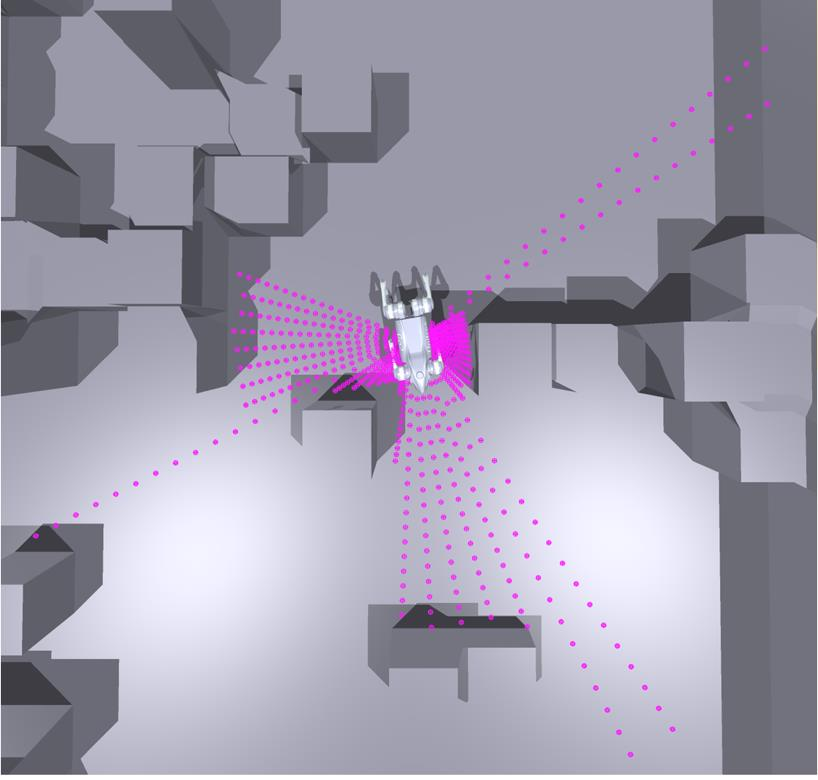
\includegraphics[width=\linewidth,height=42mm,keepaspectratio]{seanav_rays.png}\\[0.15em]
      {\scriptsize Rays that enter the robot}
    \end{column}
  \end{columns}

  \takeaway{The policy chooses the speed and also $\alpha$, how far to shift toward safety.}
\end{frame}

\begin{frame}{Contribution 1 | Safety and gradients through LSE-CBF}
  \source{Chen et al., arXiv, 2026}
  \centering
  {\footnotesize Safety condition on each ray\quad
  $h_i(x)=\rho_i-d_{\mathrm{safe}}$}

  \vspace{0.35em}
  \begin{columns}[T,onlytextwidth]
    \begin{column}{0.49\textwidth}
      \infocard[orange][24mm]{Standard CBF}{%
        \centering
        $\displaystyle h(x)=\min_{i\in\{1,\ldots,N\}} h_i(x)$\\[0.25em]
        \raggedright
        \li Switching the closest ray makes this discontinuous
        \li Gradients are hard to pass}
    \end{column}
    \hfill
    \begin{column}{0.49\textwidth}
      \infocard[blue][24mm]{LSE-CBF}{%
        \centering
        {\scriptsize $\displaystyle h(x)=-\frac1k\ln\!\Bigl(\sum_{i=1}^{N}\exp(-k\,h_i(x))\Bigr)$}\\[0.25em]
        \raggedright
        \li It is continuous, so the error reaches a bad command}
    \end{column}
  \end{columns}

  \vspace{0.35em}
  \centering
  {\footnotesize Subject to the CBF constraint $\dot h(x,u)\ge -\alpha h(x)$,\\
  move the input as little as possible into the safe set.}
  \[
    \min_{u_s}\tfrac12\|u_s-\bar{u}(x)\|^2
    \quad\text{s.t.}\quad
    \langle L_g h(x), u_s\rangle+\alpha h(x)\ge 0
  \]

  \takeaway{A plain minimum is discontinuous. LSE is continuous, so the error gets through.}
\end{frame}

\begin{frame}{Contribution 2 | Learning safe actions from the loss}
  \source{Chen et al., arXiv, 2026}
  \vspace{-0.35em}
  \[
    L_{\mathrm{total}}=L_{\mathrm{PPO}}+\lambda_{\mathrm{shield}}L_{\mathrm{shield}}+\lambda_{\mathrm{reg}}L_{\mathrm{reg}}
  \]
  \vspace{-1.55em}
  \begin{columns}[T,onlytextwidth]
    \begin{column}{0.46\textwidth}
      \infocard[blue][22mm]{$L_{\mathrm{PPO}}$}{%
        \li The loss that updates the policy
        \li Good and bad actions are learned from the critic}
      \vspace{0.22em}
      \infocard[orange][22mm]{$L_{\mathrm{shield}}$}{%
        \li Add only as much safety as needed
        \li {\scriptsize $L_{\mathrm{shield}}=\|u_{s,t}-\bar{u}_t\|^2+[\alpha_{\min}-\alpha_t]_{+}^{2}$}}
    \end{column}
    \hfill
    \begin{column}{0.52\textwidth}
      \infocard[green][\dimexpr22mm+22mm+0.22em\relax]{$L_{\mathrm{reg}}$ \ Kinematics}{%
        \li Sum of two terms
        \lieq{$L_{\mathrm{reg}}=L_{\mathrm{range}}+L_{\mathrm{smooth}}$}
        \li Speed limits
        \lieq{$L_{\mathrm{range}}=\sum_{j\in\{x,y,\omega\}}\bigl(u_{s,t}^{j}-\mathrm{clip}(u_{s,t}^{j},u_{j}^{\min},u_{j}^{\max})\bigr)^{2}$}
        \li Limit abrupt policy changes
        \lieq{$L_{\mathrm{smooth}}=\lambda_{\pi} D(\pi_{\theta}(x_t),\pi_{\theta}(\bar{x}_t))+\lambda_{V} D(V_{\phi}(x_t),V_{\phi}(\bar{x}_t))$}}
    \end{column}
  \end{columns}

  \takeaway{Regularization yields velocity commands that are safe and smooth on the real robot.}
\end{frame}

\begin{frame}{Contribution 3 | ACSI rolls back after a collision}
  \source{Chen et al., arXiv, 2026}
  {\footnotesize\color{body}
  The buffer stores the last 2 seconds, 100 steps. A collision then receives a large penalty.}

  \vspace{0.55em}
  \begin{columns}[T,onlytextwidth]
    \begin{column}{0.49\textwidth}
      \infocard[orange][18mm]{Early stop}{%
        \li $P_{\mathrm{reset}}$ ends the episode and moves on}
    \end{column}
    \hfill
    \begin{column}{0.49\textwidth}
      \infocard[blue][18mm]{Rollback}{%
        \li $P_{\mathrm{replay}}$ returns 2 seconds and retries the avoidance}
    \end{column}
  \end{columns}

  \vspace{0.4em}
  {\footnotesize\color{body} The reset rate follows the goal rate.}
  \[
    P_{\mathrm{reset}}=P_{\min}+(P_{\max}-P_{\min})\cdot\mathrm{clip}(L_{\mathrm{goal}}/1.5,\,0,\,1)
  \]

  \takeaway{Collision histories are sampled efficiently, so dangerous local scenes are learned in more detail.}
\end{frame}

\begin{frame}{Results | Simulation}
  \source{Chen et al., arXiv, 2026, Table~I}
  \centering
  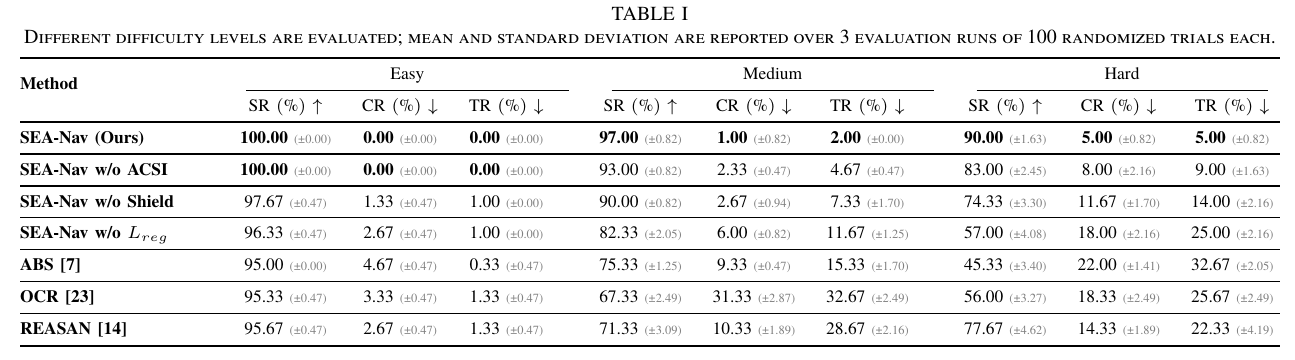
\includegraphics[width=\textwidth]{seanav_table1.png}

  \vspace{0.3em}
  {\scriptsize\color{body}
  RTX 4090, 2000 iterations, about 1 hour, in a 10\,m square. SR is success, CR is collision, and TR is timeout.\\
  On Hard, the collision rate is 5\% for SEA-Nav, 8\% without ACSI, about 12\% without the shield, and 18\% without $L_{\mathrm{reg}}$.}

  \takeaway{The gain is small on Easy and opens up on Hard, where the obstacles are dense.}
\end{frame}

\begin{frame}{Results | Real robot}
  \source{Chen et al., arXiv, 2026, Table~II, Fig.~5. Unitree Go2}
  \centering
  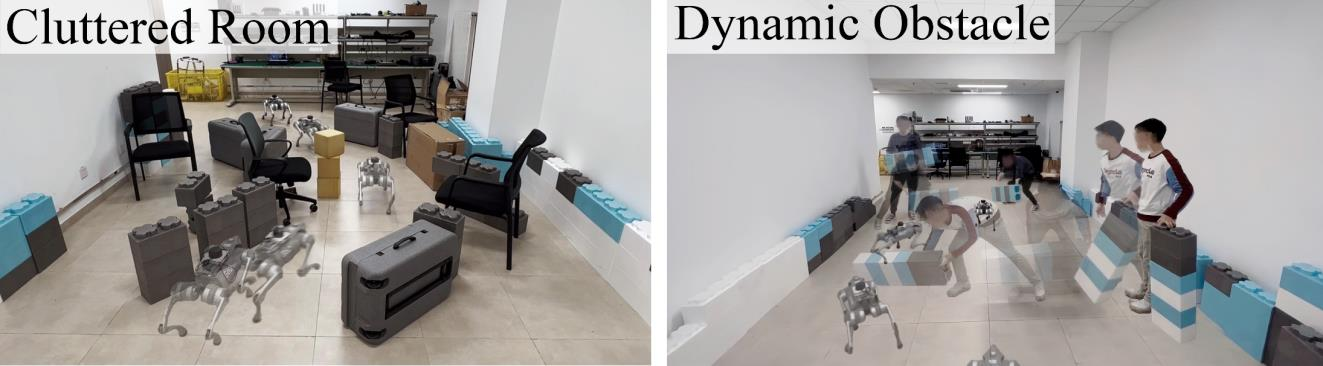
\includegraphics[width=0.49\textwidth,height=16mm,keepaspectratio]{seanav_real_ab.png}
  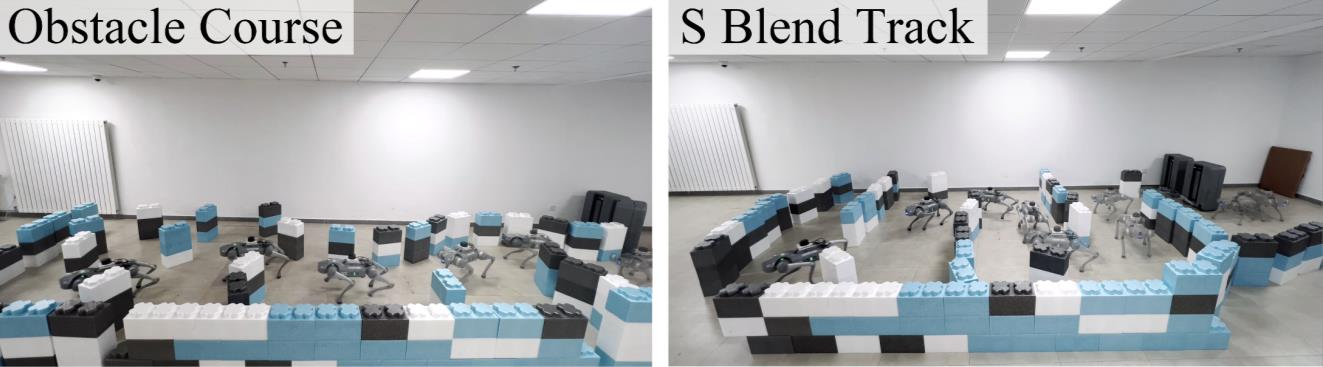
\includegraphics[width=0.49\textwidth,height=16mm,keepaspectratio]{seanav_real_cd.png}

  \vspace{0.2em}
  {\scriptsize\color{body}
  SEA-Nav uses the learned gait model. SEA-Nav-b uses Unitree's official gait model.}

  \vspace{0.15em}
  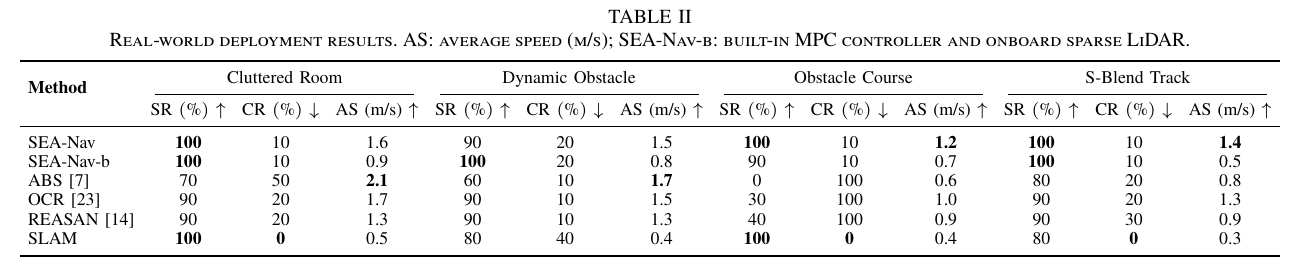
\includegraphics[width=\textwidth]{seanav_table2.png}

  \takeaway{In most scenes SEA-Nav succeeds more often, and is faster than the official model and SLAM.}
\end{frame}

\begin{frame}{Summary | SEA-Nav}
  \source{Chen et al., arXiv, 2026}
  \begin{columns}[T,onlytextwidth]
    \begin{column}{0.58\textwidth}
      \infocard[blue][15mm]{Contribution 1 | End-to-end LSE-CBF}{%
        \li Smooth the safety condition and use the same layer in training and execution. Success on Hard is 90\%.}
      \par\vspace{0.32em}
      \infocard[orange][15mm]{Contribution 2 | Kinematic regularization}{%
        \li Put speed limits and smooth changes in the loss. On the robot it runs at 1.2--1.6\,m/s.}
      \par\vspace{0.32em}
      \infocard[green][15mm]{Contribution 3 | ACSI}{%
        \li Roll back through collisions and learn. The collision rate on Hard falls to 5\%.}
    \end{column}
    \hfill
    \begin{column}{0.40\textwidth}
      \infocard[orange][48mm]{Limitations}{%
        \li Assumes flat ground
        \li Complex dead ends are not handled}
    \end{column}
  \end{columns}

  \takeaway{Safety enters as a differentiable constraint on the velocity command.}
\end{frame}

\begin{frame}{Summary | The two surveys}
  \cardbalance
  \begin{columns}[T,onlytextwidth]
    \begin{column}{0.49\textwidth}
      \infocard[green][48mm]{CATNAV | Preference}{%
        \li A VLM assigns semantic risk with no task training
        \li Similar images are cached, so there are fewer queries
        \li It looks at several paths and picks the one that matches the instruction
        \li A preference for how to walk enters as the reason for the chosen path}
    \end{column}
    \hfill
    \begin{column}{0.49\textwidth}
      \infocard[blue][48mm]{SEA-Nav | Safety}{%
        \li Learn a safe velocity command directly from the ray distances
        \li The CBF is inside the value and the loss, not a post-process
        \li Rollback after collisions teaches dense scenes in a short time
        \li Safety enters as a constraint on velocity}
    \end{column}
  \end{columns}
  \takeawaybalance{The goal is a model that has both of these properties.}
\end{frame}

\end{document}
